\documentclass[11pt,letterpaper]{article}

% Packages
\usepackage[empty]{fullpage}
\usepackage{hyperref}
\usepackage[left=0.75in,top=0.6in,right=0.75in,bottom=0.6in]{geometry}
\usepackage{titlesec}
\usepackage{enumitem}
\usepackage{xcolor}
\usepackage{fontawesome}
\usepackage{tabularx}
\usepackage{tikz}

% Define forest green color
\definecolor{forestgreen}{RGB}{34,139,34}
\definecolor{lightgreen}{RGB}{144,238,144}
\definecolor{darkgray}{RGB}{52,58,64}

% Colors for hyperlinks
\hypersetup{
    colorlinks=true,
    linkcolor=forestgreen,
    filecolor=forestgreen,
    urlcolor=forestgreen,
}

% Custom section formatting
\titleformat{\section}
{\Large\scshape\raggedright\color{forestgreen}}
{}{0em}
{}[\titlerule]
\titlespacing*{\section}{0pt}{12pt}{8pt}

% Custom commands
\newcommand{\tech}[1]{\textcolor{darkgray}{\textbf{#1}}}
\newcommand{\skill}[1]{{\small\textcolor{forestgreen}{\textbf{#1}}}}
\newcommand{\employer}[2]{{\large\textcolor{forestgreen}{\textbf{#1}}} \hfill \textbf{#2}}
\newcommand{\role}[2]{\hspace{1em}{\large\textcolor{forestgreen}{\textbf{#1}}} \hfill \textit{#2}}

% Custom bullet points
\renewcommand{\labelitemi}{$\bullet$}

% Begin document
\begin{document}

% Header
\begin{center}
{\Huge \textcolor{forestgreen}{\textbf{Andrew G. Gurik}}}\\[5pt]
{\large \href{mailto:andrewgurik@gmail.com}{\faEnvelope\ andrewgurik@gmail.com} \textcolor{forestgreen}{$\bullet$} 
\faPhone\ (309) 868-4405 \textcolor{forestgreen}{$\bullet$} 
\faMapMarker\ Ames, IA}\\[10pt]
\end{center}

% Core Competencies
\section{Core Competencies}
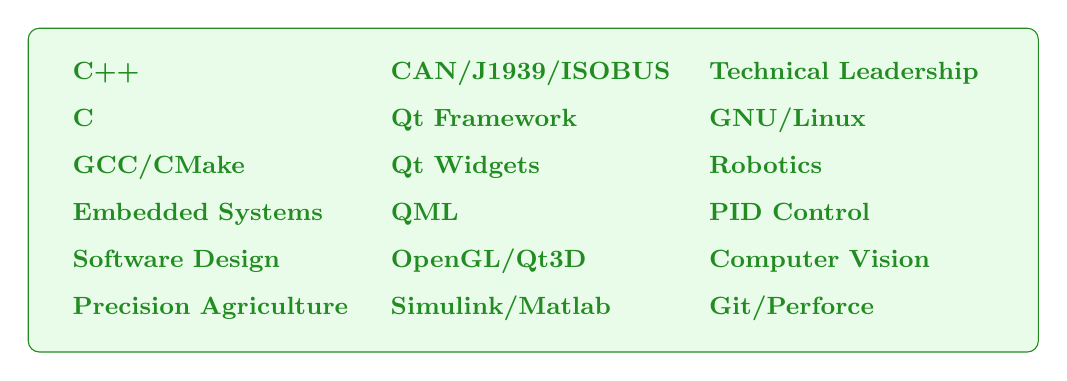
\begin{tikzpicture}
\node[rectangle,draw=forestgreen,rounded corners,inner sep=10pt,fill=lightgreen!20,text width=\textwidth] {
\begin{tabularx}{\textwidth}{XXX}
\skill{C++} & \skill{CAN/J1939/ISOBUS} & \skill{Technical Leadership} \\[5pt]
\skill{C} & \skill{Qt Framework} & \skill{GNU/Linux} \\[5pt]
\skill{GCC/CMake} & \skill{Qt Widgets} & \skill{Robotics} \\[5pt]
\skill{Embedded Systems} & \skill{QML} & \skill{PID Control} \\[5pt]
\skill{Software Design} & \skill{OpenGL/Qt3D} & \skill{Computer Vision} \\[5pt]
\skill{Precision Agriculture} & \skill{Simulink/Matlab} & \skill{Git/Perforce}
\end{tabularx}
};
\end{tikzpicture}

% Experience Section
\section{Experience}

% Add some vertical space before first company
\vspace{2pt}
\employer{Ag Leader Technology}{2018 - present}\\[3pt]

\role{Staff Software Engineer}{2023 - present}
\begin{itemize}[leftmargin=*,itemsep=2pt]
\item Lead development of next-generation precision agriculture displays, implementing advanced \tech{3D geospatial mapping engine} using \tech{Qt3D} and \tech{OpenGL} in an \tech{embedded Linux} environment
\item Architect and implement automated grain cart alignment system using \tech{computer vision} (\tech{VPI AprilTag}) on \tech{NVIDIA Jetson Orin Nano SOM}
\item Drive technical direction and mentor team members in modern \tech{C++}, \tech{embedded systems}, and \tech{real-time graphics}
\end{itemize}


\role{Senior Software Engineer}{2021 - 2023}
\begin{itemize}[leftmargin=*,itemsep=2pt]
\item Led Scrum team developing precision agriculture software for in-cab displays and \tech{CAN bus} (\tech{J1939}) connected modules
\item Designed and implemented precision nozzle-control spraying system, including touch UI, \tech{CAN protocol}, \tech{embedded architecture}, and \tech{PID control systems}
\item Spearheaded next-generation product development, focusing on \tech{real-time performance} and \tech{user experience}
\end{itemize}


\role{Software Engineer}{2018 - 2021}
\begin{itemize}[leftmargin=*,itemsep=2pt]
\item Developed software for precision agriculture displays using \tech{Qt/QML} and \tech{C++} with \tech{CAN bus} (\tech{J1939} \& \tech{ISOBUS})
\item Created high-speed planting system with real-time control and monitoring
\item Maintained critical systems including planter downforce and ISOBUS dry spreader
\end{itemize}

\vspace{8pt}
\employer{Randstad Technologies}{2017 - 2018}\\[3pt]

\role{Software Engineer}{} -- (Caterpillar) Core Machine Software
\begin{itemize}[leftmargin=*,itemsep=2pt]
\item Enhanced Virtual Platform ecosystem with \tech{Simulink}, \tech{Python}, \tech{C\#}, and \tech{C++} tooling
\item Implemented \tech{Google Test} infrastructure for automated testing
\item Developed cross-application testing framework for machine software validation
\end{itemize}

\vspace{8pt}
\employer{Caterpillar, Inc.}{2013 - 2016}\\[3pt]
\role{Software Engineer}{}\\[2pt]
\textit{Core Machine Software}
\begin{itemize}[leftmargin=*,itemsep=2pt]
\item Developed Windows-based transmission control simulation environment
\item Designed scalable architecture supporting hundreds of applications across product lines
\item Integrated virtual \tech{CAN Bus} simulation with comprehensive testing framework
\end{itemize}

\textit{Drivetrain Systems \& Software - Large Mining Trucks}
\begin{itemize}[leftmargin=*,itemsep=2pt]
\item Led development of embedded control systems for hydraulic transmissions
\item Managed global development teams and implemented \tech{CI/CD} practices
\item Pioneered simulation and software-in-loop testing methodologies
\end{itemize}

% Education Section
\section{Education}
{\large\textcolor{forestgreen}{\textbf{B.S. Electrical Engineering}}} \hfill Iowa State University, 2012

\end{document}
